\newcommand{\mb}[1]{\mathbb{#1}}
\newcommand{\conv}{\operatorname{conv}}

\task{Уйдём на Север}
Снежная Королева возвращается обратно на Север и собирает чемоданы. За то время, что она провела вне дома, она накопила множество льдинок самой разной формы и хочет их все взять с собой. Помогите Снежной Королеве быстрее собрать вещи.

\begin{enumerate}
\item У Снежной Королевы есть стеллаж с плоскими квадратными чемоданами и множество льдинок треугольной формы, которыми она дорожит. Какова наименьшая сторона плоского квадратного чемодана, в которую поместятся одновременно две плоские льдинки в форме равнобедренных прямоугольных треугольников с длинами катетов $a$ и $b$, соответственно? А две льдинки в форме равносторонних треугольников? В плоские чемоданы льдинки укладываются только в один слой.
\begin{figure}[h]
\begin{center}

\begin{tikzpicture}[ xscale=0.7, yscale=0.7]

\draw (0,0) -- (2,0) --  (2,2) -- (0,2) -- (0,0);
\path  [fill=cyan] (0,0) -- (1,1.5) --  (2,0.5) -- (0,0);
\path  [fill=cyan] (0,1) -- (1,2) --  (0.5,0.9) -- (0,1);

\end{tikzpicture}
\end{center}
\caption{Две треугольные льдинки в не самом подходящем плоском квадратном чемодане}
\end{figure}
\item Настала очередь прозрачных картин изо льда. В какой плоский квадратный чемодан поместятся две ледяные квадратные картины со сторонами $a$ и $b$, соответственно?
\item Стеллаж с квадратными чемоданами опустел. Но в ящике комода обнаружились чемоданы самых разных форм. Первыми на глаза попалась стопка с несчётным числом плоских прямоугольных чемоданов. Как выглядят прямоугольные чемоданы наименьшей площади, в которые можно поместить льдинки уже рассмотренных форм?
\item Для ускорения сборов удобнее класть более двух льдинок в чемодан. В какой прямоугольный чемодан лучше всего убрать $3$ одинаковые равносторонние льдинки? А $4$? Что будет в случае льдинок --- прямоугольных треугольников?
\item Кубические чемоданы отлично подходят для упаковки объёмных льдинок-тетраэдров. Решите задачу для различных пар таких льдинок.
\item Рассмотрите льдинки и чемоданы других форм. Например, круглые льдинки-тарелки и треугольные чемоданы.
\end{enumerate}


\task{Вас снимают}

Пусть $I\subseteq \mb R$ является объединением непересекающихся отрезков на прямой. Обозначим за $L(I)$ длину множества $I$, то есть сумму длин соответствующих отрезков. Подмножество плоскости $A$ будем называть фигурой, если оно ограничено, замкнуто и его пересечение с любой прямой есть объединение конечного числа отрезков (определения \ref{closed} и \ref{bounded} ниже). В частности, любой многоугольник является фигурой. Зафиксируем некоторую декартову систему координат на плоскости. Для фигуры $A$ определим её $x$-снимок, как функцию $f_x\colon \mb R\to \mb R$, которая по точке $t$ на прямой $OX$  вычисляет длину пересечения $A$ с прямой, проходящей через $t$ и перпендикулярной $OX$ 
$$f_x(t)=L(A\cap \{(t,y)\in\mb R^2\,|\, y\text{ любое}\}).$$

Аналогично определим $y$-снимок фигуры $A$ как

$$f_y(t)=L(A\cap \{(x,t)\in\mb R^2\,|\, x\text{ любое}\}).$$

\begin{enumerate}
\item Какая фигура обладает следующими $x$- и $y$-снимками:
$$f_x(t)= f_y(t)=\begin{cases}
0, &t\leq 0\\
\tfrac{7t}{12}, &0\leq t\leq 3\\
\tfrac{21}{12}, &3\leq t\leq 4\\
-\tfrac{7t}{12}+ \tfrac{49}{12},&4\leq t\leq 8\\
0,& 8\leq t
\end{cases} \,\,\,\,?$$

\item Найдите способ восстановить фигуру $A$, а также варианты её расположения по $x$- и $y$-снимкам, если известно, что \\
а) $A$ --- некоторый прямоугольник;\\
б) $A$ --- некоторый треугольник;\\
в) $A$ --- некоторый четырёхугольник.\\
Можно ли обойтись только одним снимком?

\item Приведите пример двух неравных фигур на плоскости, имеющих одинаковые $x$- и $y$-снимки.
\item Пусть $A$ некоторая фигура. Можно ли восстановить и, если можно, то как, по $x$- и $y$-снимкам следующую информацию:\\
а) $A$ имеет площадь $S$;\\
б) $A$ является невыпуклой фигурой (см. определение \ref{convex}); \\
в) $A$ является многоугольником с $n$ вершинами;\\
г) $A$ содержит фиксированную точку $(x_0,y_0)$?\\
Можно ли добиться ответов на эти вопросы, если заранее известна дополнительная информация про $A$? Например, если известно, что $A$ выпуклая и центрально-симметричная фигура?
\item Повернём исходную систему координат относительно начала отсчёта на угол $\alpha$ против часовой стрелки. $x$-снимок в новой  системе координат назовём $\alpha$-снимком. Так например, $0$-снимок это $x$-снимок, $\frac{\text{π}}{2}$-снимок это $y$-снимок.
Исследуйте предыдущие пункты, если вместо $x$- и $y$- снимков даны $\alpha$- и $\beta$-снимки, для некоторых неравных углов $\alpha$ и $\beta$? Можно ли узнать дополнительную информацию (например, восстановить любую фигуру), если даны три разных снимка?
\end{enumerate}


\task{Целые структуры}
\begin{enumerate}
\item Пусть даны два целых числа $a$ и $b$. Множеством, подчинённым $a$ и $b$ назовём $S$, подмножество в $\mb Z$, удовлетворяющее свойствам:\\
а) $a,b\in S$;\\
б) Для любого $x\in S$ число $-x$ лежит в $S$;\\
в) Для всех $x$ и $y$ из $S$ число $ax+by$ также лежит в $S$.\\
Пусть $a=2$, а $b=3$. Покажите, что любое подчинённое $2$ и $3$ множество $S$ обязательно содержит 1.
\item Опишите наименьшее множество $S$, подчинённое $a$ и $b$, если $a=b=1$. Что будет, если $a=2$, $b=3$?
\item Рассмотрите аналогичную задачу для $a=4$, $b=5$.
\item При каком условии на $a$ и $b$ в любом $a,b$-подчинённом множестве $S$ найдётся число, имеющее остаток $k$ по модулю $n$ для всех $0 \leq k<n$.
\item Пусть $a$ и $b$ взаимно просты. Покажите, что любое подчинённое $a$ и $b$ множество содержит 1.
\item Натуральной плотностью множества $A\subseteq \mb Z$ назовём предел отношения 
$$ \lim_{n\to \text{inf\,}ty}\frac{|\{x\in A\,|\, -n\leq x\leq n\}|}{2n},$$ 
если этот предел существует. Верно ли, что для не взаимно простых $a$ и $b$ размер наименьшего подчинённого $a$ и $b$ множества имеет натуральную плотность 0?
\end{enumerate}


\task{Задача №4 Буйство красок}
Известный художник Петров имеет следующую манеру письма: он разбивает квадратный холст $n\times n$ на квадратики $1\times 1$, после чего каждый квадратик закрашивает в один из $k$ цветов, имеющихся в наличии. Так как на картине не указан верх и низ, то искусствоведы и сам Петров считают две картины, отличающиеся поворотом на $90^{\circ}$, одинаковыми.
\begin{enumerate}
\item В детстве Петров писал на холсте $2\times 2$. Известно, что за это время он написал более 100, но менее 200 различных картин, при этом с холстов $2\times 2$ на большие он перешёл после того, как написал картины размера $2\times 2$ всеми доступными ему способами. Сколько красок было у Петрова в детстве? Сколько в точности картин $2\times 2$ он написал?

\begin{figure}[h]
\begin{center}
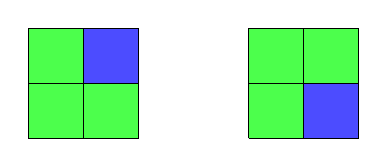
\begin{tikzpicture}[ xscale=0.7, yscale=0.7]

\path  [fill=white!30!green] (0,0) -- (2,0) --  (2,1) -- (1,1) -- (1,2) -- (0,2) -- (0,0);
\path  [fill=white!30!blue] (1,1) -- (1,2) -- (2,2) -- (2,1) -- (1,1);

\path  [fill=white!30!green] (4,0) -- (5,0) --  (5,1) -- (6,1) -- (6,2) -- (4,2) -- (4,0);
\path  [fill=white!30!blue] (5,0) -- (6,0) -- (6,1) -- (5,1) -- (5,0);
\draw (0,0) -- (2,0) --  (2,2) -- (0,2) -- (0,0);
\draw (1,0) -- (1,2);
\draw (0,1) -- (2,1);
\draw (4,0) -- (6,0) --  (6,2) -- (4,2) -- (4,0);
\draw (5,0) -- (5,2);
\draw (4,1) -- (6,1);

\end{tikzpicture}
\end{center}
\caption{Две неразличимые детские картины Петрова $2\times 2$ на двух цветах}
\end{figure}

\item Обретя популярность, Петров переключился на масштабные проекты с холстами $n\times n$, $n\geq 3$ и числом красок $k$. Найдите асимптотику или формулу для числа различных картин, которые мог написать Петров на полотнах $3\times 3$, $4\times 4$, при $k\to\text{inf\,}ty$. Оцените число возможных картин Петрова при других $n$ или дайте точную формулу.
\item Для систематизации картин Петрова искусствоведы предложили несколько классификаций, основанных на том, что две картины Петрова не стоит различать, если они отличаются цепочкой определённых преобразований. Найдите конкретные значения, оцените при больших $n$ и $k$ или дайте точную формулу числа работ Петрова по классификациям, основанным на преобразованиях: \\
а) Поворот на $90^{\circ}$ и отражения относительно осей симметрии квадрата;\\
б) Преобразования из пункта а) и преобразование, сдвигающее все строчки квадрата, кроме первой, на 1 вниз, а нижнюю строчку ставящее наверх.\\
в) Преобразования из пункта а) и преобразования, меняющие цвета на картине: цвет $i$ на цвет $j$, цвет $j$ на цвет $i$, и не меняющее остальные цвета. Назовём такие преобразования элементарными перекрашиваниями.\\
г) Преобразования из пункта а) и преобразования, позволяющие в одном из столбцов сдвинуть все квадратики на 1 по циклу. \\
\begin{figure}[h]\label{recolor}
\begin{center}
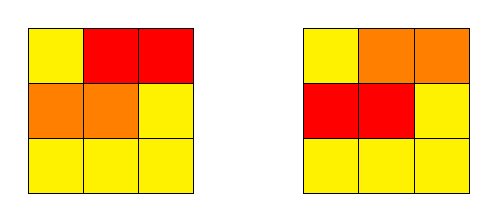
\begin{tikzpicture}[ xscale=0.7, yscale=0.7]

\path  [fill=yellow] (0,0) -- (3,0) --  (3,3) -- (0,3) -- (0,0);
\path  [fill=yellow] (5,0) -- (8,0) --  (8,3) -- (5,3) -- (5,0);

\path  [fill=orange] (0,1) -- (2,1) --  (2,2) -- (0,2) -- (0,1);
\path  [fill=red] (5,1) -- (7,1) --  (7,2) -- (5,2) -- (5,1);

\path  [fill=red] (1,2) -- (3,2) --  (3,3) -- (1,3) -- (1,2);
\path  [fill=orange] (6,2) -- (8,2) --  (8,3) -- (6,3) -- (6,2);

\foreach \n in {0,...,3}{\draw (0,\n) -- (3,\n);}

\foreach \m in {0,...,3}{\draw (\m,0) -- (\m,3);}

\foreach \n in {0,...,3}{\draw (5,\n) -- (8,\n);}

\foreach \m in {5,...,8}{\draw (\m,0) -- (\m,3);}

\end{tikzpicture}
\end{center}
\caption{Картины, отличающиеся заменой оранжевого и красного цветов}
\end{figure}
\item Художник Иванов решил превзойти Петрова и стал разбивать равносторонний треугольник со стороной $n$ на треугольники со стороной 1 и раскрашивать их в $k$ цветов. Исследуйте аналогичный предыдущим пунктам вопрос. В частности, рассмотрите классификации, разрешающие преобразования: \\
а) Поворот на $120^{\circ}$;\\
б) Поворот на $120^{\circ}$ и отражения относительно осей симметрии треугольника;\\
в) Преобразования из пункта б) и элементарные перекрашивания;\\
г) Преобразования из пункта а) и преобразование, сдвигающее по циклу цвета в одном горизонтальном ряду большого треугольника.
\item Рассмотрите другие, в том числе трёхмерные, разбиения и их раскраски. Придумайте другие классификации.

\end{enumerate}



\task{Дискретная непрерывность}
 Будем говорить, что два целых числа $a$ и $b$ соседние, если $|a-b|\leq 1$. Пусть $I$ --- некоторое подмножество внутри целых чисел. Отображение $f:I\to \mb Z$ назовём дискретно непрерывным, если для любых двух соседних чисел $a,b\in I$ их образы $f(a)$ и $f(b)$ тоже соседние. 

\begin{enumerate}

\item Пусть $a<b$ --- два целых числа. Целочисленным отрезком $[a,b]$ будем называть подмножество целых чисел $[a,b]=\{x\in \mb Z\,| \, a\leq x\leq b\}$. Пусть дано  дискретно-непрерывное отображение $f\colon \mb Z\to \mb Z$. Покажите, что для любого целого числа $x \in [f(a),f(b)]$ существует $c$, такое, что $a\leq c\leq b$ и $f(c)=x$.

\item
Пусть $n\in \mb N$ --- некоторое натуральное число. Рассмотрим функцию $\rho_1(x,y)\colon \mb Z^n\times \mb Z^n \to \mb R$, заданную по правилу
$$\rho_1(x,y)=\sum_{i=1}^n |x_i-y_i|, \text{ где $x=(x_1,\dots, x_n)$, а $y=(y_1,\dots, y_n)$.}$$

Будем говорить, что точки $x$, $y\in \mb Z^n$ соседние, если $\rho_1(a,b)\leq 1$. Пусть $A$ --- подмножество в $\mb Z^n$, а $k\in \mb N$. Отображение $f\colon A \to \mb Z^k$ назовём дискретно-непрерывным, если для любых соседних $x$, $y\in A$ их образы $f(x)$ и $f(y)$ соседние в $\mb Z^k$. 
Для каждого натурального числа $m$ определим множества 
$$D^{n}_m=\{x\in \mb Z^n\,|\, |x_i|\leq m\} \,\,\text{ и }\,\, S^{n-1}_m=\{x\in D^{n}_m\,|\,\exists i\leq n\,\, |x_i|= r\}.$$ 

Пусть дискретно-непрерывное отображение $f\colon S^1_m \to \mb Z^{2}$, а $x\in \mb Z^2$ не лежит в $f(S^1_m)$. Для любого луча $l$, исходящего из точки $x$ и не содержащего точек $f(S^1_m)$, можно определить  число $i_{l,f}$ его пересечений с ломаной, построенной по $f$. Сделаем это следующим образом:
 
$$i_{l,f}=\frac{1}{2}\big|\{ (a,b)\, | \,a,\, b\in S^1_m ,\,\, \rho_1(a,b)=1 \text{ и $l$ пересекает отрезок, соединяющий $f(a)$ и $f(b)$} \}\big|.$$

Число $\frac{1}{2}$ появляется из-за того, что одно и тоже пересечение соответствует и паре $(a,b)$, и паре $(b,a)$. Покажите, что чётность $i_{l,f}$  не зависит от выбора $l$ и, следовательно, является характеристикой точки $x$.
\begin{figure}[hh]
\begin{center}
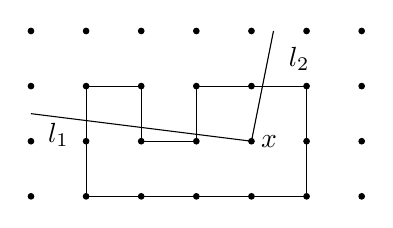
\begin{tikzpicture}[ xscale=0.7, yscale=0.7]

\draw (0,0) -- (4,0) -- (4,2) -- (2,2) -- (2,1) -- (1,1) -- (1,2) -- (0,2) -- (0,0);
\draw (3,1) -- (-1, 1.5);
\draw (3,1) -- (3.4, 3);
\foreach \n in {-1,...,5}{
\foreach \m in {0,...,3}{\draw [fill] (\n,\m) circle [radius=0.05] ;}
}
\node [below] at (-0.5, 1.5) {$l_1$};
\node [right] at (3.5, 2.5) {$l_2$};
\node [right] at (3, 1) {$x$};
\end{tikzpicture}
\end{center}
\caption{Ломаная и два луча, исходящие из одной точки, с $i_{l_1,f}=3$ и $i_{l_2,f}=1$}
\end{figure}

\item  Точку $x\in \mb Z^2$, не лежащую в $f(S^1_m)$, назовём внутренней по отношению к $f$, если $i_{l,f}$ нечётно, и внешней, если $i_{l,f}$ чётно. Пусть дано дискретно-непрерывное отображение $g\colon D^2_m\to \mb Z^{2}$. Положим $f=g|_{S^1_m}$ --- сужение отображения $g$. Покажите, что для любой $f$-внутренней точки $x$ существует $y\in D_k^2$, что $g(y)=x$. 

\item
Определим метрические пространства (см. \hyperref[metric]{метрика})  $\mb Z^{n,p}$, где $p=\text{inf\,}ty$, или  $p\geq 1$ --- вещественное число, следующим образом:
$$ \mb Z^{n,{\text{inf\,}ty}}=(\mb Z^n, \max\{|x_i-y_i| \, \colon\, i \in \overline{1,n}\}) \, \text{ и при $p$ вещественном } \,\mb Z^{n,p}=\left(\mb Z^n, \rho_p \right),$$
где  $\rho_p(x,y)=(\sum_{1\leq i\leq n} {|x_i-y_i|}^p)^{1/p}$.  Заметим, что если $n=1$, то все  метрики $\rho_p$ совпадают, поэтому при $n=1$ индекс $p$ можно опустить. Естественным образом, расстояние ограничивается и на подмножества указанных метрических пространств.
Определение понятия $L$-липшицевого отображения можно найти в конце (см. определение \ref{lip}).
\begin{description}
\item[а)] Покажите, что 1-липшицевы отображения из $\mb Z^{n,1} \to \mb Z^{k,1}$ являются дискретно-непрерывными и наоборот.
\item[б)] Опишите все пары чисел $L_1$ и $L_2$, такие что  отображение $f\colon \mb Z^{2,p} \to \mb Z^{2,p}$ липшицево с константой $L_1$ тогда и только тогда, когда оно $L_2$-липшицево.
\item[в)] Исследуйте взаимосвязь между условиями липшицевости для отображений $f\colon \mb Z^2 \to \mb Z^2$ в метриках $\rho_p$ и $\rho_q$ с различными константами $L$. 
\end{description}

\item Пусть $L$ --- натуральное число. Покажите, что для любого $L$-липшицевого отображения $f\colon \mb Z \to \mb Z$ и любого целочисленного отрезка $[a,b]$
$$\frac{|f([a,b])|}{|\conv(f([a,b]))|}\geq \frac{1}{L},$$
где $|f([a,b])|$ --- это количество точек в образе $[a,b]$, а $\conv(f([a,b]))$ --- наименьший отрезок, содержащий $f([a,b])$.

\item Зададим расстояние на $D^n_m$ c помощью метрики $\rho_1$. Сформулируйте и докажите аналог пункта 6 задачи для $L$-липшицевых отображений из $D^2_m\to \mb Z^{2,q}$.
\item Обобщите все указанные теоремы на случай размерности больше 2. Опишите все $L$-липшицевы биекции из $\mb Z^{n,p} \to \mb Z^{n,q}$ для маленьких $L$.
\end{enumerate}





\task{Гипергеометрическая прогрессия}
\begin{enumerate}
\item Рассмотрим следующее рекуррентное соотношение:
$$p(n)a_{n}=q(n)a_{n-1}, \text{ для $n> n_0$ и } a_{n_0}=\lambda,$$
где $\lambda$ --- некоторое вещественное число, а $p(n)$ и $q(n)$ --- некоторые многочлены с вещественными коэффициентами. Выведите явную формулу для его решения.
\item Последовательность из предыдущего пункта назовём гипергеометрической прогрессией. Будем говорить, что многочлены $p$ и $q$ определяют эту прогрессию.  Являются или нет частными случаями гипергеометрической прогрессии: а) геометрическая прогрессия; б) арифметическая прогрессия; в) $a_n=n!$; г) $a_n=C_n^k$ для фиксированного $k$; д) $a_n= \tfrac{(-1)^n+1}{2}$? Если да, то какие многочлены их задают?
\item Рассмотрим рекуррентное соотношение 
$$p(n)a_{n}=q(n)a_{n-1} +r(n)a_{n-2},$$
где $p(n)$, $q(n)$, $r(n)$ --- некоторые многочлены. При каких $p$, $q$ и $r$ у такого рекуррентного соотношения нет решений в виде гипергеометрической прогрессии? 
\item Исследуйте предыдущий вопрос для соотношения 
$$p_0(n)a_{n}=p_1(n)a_{n-1} + p_2(n)a_{n-2}+\cdots+p_k(n-k)a_{n-k},$$
где $k$ фиксировано, $p_i(n)$ --- некоторые многочлены.
\item Пусть даны две гипергеометрические прогрессии $a_n$ и $b_n$. При каких условиях на многочлены, задающие $a_n$ и $b_n$, существуют числа $r_1(n)$ и $r_2(n)$, что $r_1(n) a_n + r_2(n) b_n=0$ для всех $n$? 
\item Исследуйте предыдущий вопрос для большего числа гипергеометрических прогрессий.
\item Пусть $a_n$ и $b_n$ --- две последовательности. Определим последовательность $a*b_n$ равенством 
$$a*b_n=\sum_{0\leq i\leq n} a_i b_{n-i}.$$
Предположим, что $a_n$ и $b_n$ --- гипергеометрические прогрессии. Всегда ли последовательность $a*b_n$ есть конечная сумма гипергеометрических прогрессий?  Если нет, то какие условия надо наложить на $a_n$ и $b_n$, чтобы это было верно? Начните со случая геометрических прогрессий.
\item Исследуйте существование решений в виде гипергеометрических функций для рекуррентного соотношения 
$$p(0,n)a_{n}=p(1,n)a_{n-1} +\cdots+p(k,n-k)a_{n-k}+ \cdots + p(n_0,n-n_0)a_{n_0},$$
где $p(n,k)$ --- гипергеометрическая функция по $n$ и по $k$.
\end{enumerate}


\task{Зависимые матрицы}

\begin{enumerate}
\item Пусть $B$, $C$ и $D$ матрицы $2\times 2$ с коэффициентами из $\mb R$ (см. определение \ref{matrix} ниже). Линейным уравнением в матрицах относительно матрицы $X$ назовём уравнение вида: 
$$CXD=B.$$
Матрица $A\in M_2(\mb R)$ называется его решением, если 
$$C\cdot A\cdot D=B,$$
где $\cdot$ обозначает произведение матриц (см. определение \ref{product}). Обозначение произведения для краткости будем опускать.
Решите уравнение:
$$\left(\begin{smallmatrix} 1&2\\ 0&1 \end{smallmatrix}\right) X \left(\begin{smallmatrix} 3&1\\ 1&0 \end{smallmatrix}\right) =
\left(\begin{smallmatrix} 5&1\\ 5&2 \end{smallmatrix}\right) .$$
\item Покажите, что уравнение $CXD=B$ разрешимо тогда и только тогда, когда разрешимы уравнения $CX=B$ и $XD=B$. При каких условиях на $C$ и $D$ уравнение $CXD=B$ разрешимо при любых $B$?
\item Естественным образом, можно определить обобщённые линейные уравнения:
$$C_1 X D_1+ C_2 X D_2+\dots+ C_n X D_n=B.$$
Исследуйте разрешимость таких уравнение для любых $B$ и решите обобщённое линейное уравнение:
$$\left(\begin{smallmatrix} 1&1\\ 1&2 \end{smallmatrix}\right) X \left(\begin{smallmatrix} 2&1\\ 1&0 \end{smallmatrix}\right) + \left(\begin{smallmatrix} 1&-1\\ 0&1 \end{smallmatrix}\right) X \left(\begin{smallmatrix} 1&1\\ 0&1 \end{smallmatrix}\right) =
\left(\begin{smallmatrix} 5&1\\ 5&2 \end{smallmatrix}\right).$$
\item Последовательность матриц вида $A_n=C^nA_0$ назовём геометрической прогрессией. Опишите все решения линейного рекуррентного соотношения $A_{n+1}=CA_nD$, являющиеся геометрическими прогрессиями. Можно ли любое решение такого рекуррентного соотношения представить в виде суммы геометрических прогрессий? В частности, ответьте на указанные вопросы для соотношения
$$A_{n+1}=\left(\begin{smallmatrix} 1&2\\ 0&1 \end{smallmatrix}\right) A_n \left(\begin{smallmatrix} 3&1\\ 1&0 \end{smallmatrix}\right).$$
\item Исследуйте аналогичный вопрос для рекуррентных соотношений вида $A_{n+1}=CA_n+A_nD$.
\item Рассмотрите рекуррентное соотношение $A_{n+1}=C_1A_nD_1+C_2A_nD_2$. Исследуйте существование у этого рекуррентного соотношения решения в виде геометрической прогрессии. В частности, опишите все решения, являющиеся геометрическими прогрессиями для соотношения 
$$A_{n+1}=\left(\begin{smallmatrix} 1&1\\ 1&2 \end{smallmatrix}\right) A_n \left(\begin{smallmatrix} 2&1\\ 1&0 \end{smallmatrix}\right) + \left(\begin{smallmatrix} 1&-1\\ 0&1 \end{smallmatrix}\right) A_n \left(\begin{smallmatrix} 1&1\\ 0&1 \end{smallmatrix}\right).$$
\item Исследуйте выразимость в геометрических прогрессиях  решений линейных рекуррентных соотношений вида
$$A_{n+1}=C_1A_nD_1+ C_2 A_{n-1}D_2,$$
а также линейных рекуррентных соотношений большего порядка.
\end{enumerate}




\task{Можно ли разрезать?}
\begin{enumerate}
\item Пусть $\varphi$ --- некоторый угол. Покажите, что 
$$\cos n\varphi=p(\cos\varphi),$$
где $p(x)$ --- это многочлен степени $n$ с целыми коэффициентами.
\item Покажите, что угол между гипотенузой и катетом в прямоугольном треугольнике со сторонами 3, 4, 5 не равен:\\
а) $\tfrac{k\text{π}}{5}$, где $k$ --- целое;   б) $\tfrac{k\text{π}}{l}$, где $k$ и $l$ --- целые неотрицательные числа.
\item Можно ли так изобразить равносторонний треугольник на координатной плоскости, чтобы координаты вершин являлись рациональными числами?
\item Опишите все треугольники с рациональными координатами вершин и углами вида $\tfrac{k\text{π}}{l}$, где $k$ и $l$ --- целые неотрицательные числа. Такие углы в дальнейшем будем называть рациональными.
\item Разрезанием многоугольника $P$ назовём такой набор многоугольников $P_i$, где $1\leq i\leq n$ внутри $P$, что $P=\bigcup_{1\leq i\leq n} P_i$ и при $i\neq j$ многоугольники $P_i$ и $P_j$ могут пересекаться лишь по точкам на границе.
Пусть дан прямоугольник $ABCD$ со сторонами $a$ и $b$. Опишите все $a$ и $b$, при которых его можно разрезать на три треугольника с рациональными углами. Приведите примеры разрезаемых и неразрезаемых прямоугольников.
\item Найдите критерий, при котором многоугольник может быть разрезан каким-либо образом на треугольники с рациональными углами.
\item Два многоугольника $P$ и $Q$ с рациональными углами,  назовём рационально равносоставленными, если существует разрезание $\{P_i\}_{i\in \overline{1,n}}$ для $P$ и разрезание $\{Q_i\}_{i\in \overline{1,n}}$ для $Q$, такие что фигуры $P_i$ и $Q_i$ равны и имеют рациональные углы для всех $i$. Например, 
\begin{figure}[h]
\begin{center}
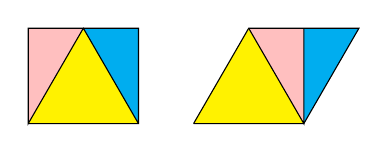
\begin{tikzpicture}[xscale=0.7, yscale=0.7]

\path[fill=yellow] (0,0) -- (2,0) -- (1, 1.73) -- (0,0);
\path[fill=pink] (0,0) -- (1, 1.73) -- (0, 1.73) -- (0,0);
\path[fill=cyan] (2,0) -- (1, 1.73) -- (2, 1.73) -- (2,0);

\path[fill=yellow] (3,0) -- (5,0) -- (4, 1.73) -- (3,0);
\path[fill=pink] (5,0) -- (4, 1.73) -- (5, 1.73) -- (5,0);
\path[fill=cyan] (5,0) -- (6, 1.73) -- (5, 1.73) -- (5,0);

\draw (0,0) -- (2,0) -- (2,1.73) -- (0,1.73) -- (0,0) -- (1,1.73) -- (2,0);
\draw (3,0) -- (5,0) -- (6,1.73) -- (4,1.73) -- (3,0) ;
\draw (4, 1.73) -- (5, 0) -- (5,1.73);
\end{tikzpicture}
\end{center}
\caption{Разрезание на попарно равные треугольники с рациональными углами.}
\end{figure}

Найдите необходимые и достаточные условия рациональной равносоставленности двух фигур. Приведите примеры рационально равносоставленных и не рационально равносоставленных многоугольников.
\end{enumerate}






\task{Порядки}
Пусть $M_1$ и $M_2$ --- два упорядоченных множества (см. определение \ref{order}). Отображение $f\colon M_1 \to M_2$ называется монотонным, если для любых $x$ и $y$ из $M_1$, таких, что $x\leq y$, выполнено, что $f(x)\leq f(y)$ относительно порядка на $M_2$. Монотонное отображение $f\colon M_1\to M_2$ называется изоморфизмом, если $f$ биективно и обратное отображение $f^{-1}\colon M_2 \to M_1$ также монотонно.
\begin{enumerate}
\item Пусть $f\colon M \to N$ --- изоморфизм двух упорядоченных множеств. Покажите, что для любого $x\in M$ множество $M_{\leq x}=\{y\in M\,|\, y\leq x\}$  изоморфно  $N_{\leq f(x)}=\{y\in N\,|\, y\leq f(x)\}$. 
\item Опишите все изоморфизмы из $\mathcal P(X) \to \mathcal P(X)$, где $\mathcal P(X)$ --- множество всех подмножеств множества $X$, упорядоченных по отношению включения $\subseteq$.
\item Пусть $M_1$ и $M_2$ --- два упорядоченных множества. Тогда введём на $M_1\times M_2$ порядок следующим образом:
 $$(x_1, y_1)\leq_{nat} (x_2,y_2) \text{ тогда и только тогда, когда } x_1\leq x_2 \text{ и } y_1\leq y_2.$$
Обозначим получившееся упорядоченное множество как $M_1\times_{nat}M_2$. Будем называть такой порядок естественным. Введём на $M_1\times M_2$ другой порядок:
\begin{align*}
(x_1, y_1)\leq_{lex} (x_2,y_2) & \Longleftrightarrow \\
\Longleftrightarrow\ \ & x_1< x_2\\
\text{или}\ \ & x_1=x_2 \text{ и } y_1\leq y_2 \\
\end{align*}
Обозначим это упорядоченное множество как $M_1\times_{lex} M_2$.

Покажите, что следующие упорядоченные множества не изоморфны между собой: $\mb N$, $\mb Z$, $\mb N\times_{nat} \mb N$, $\mb N\times_{lex} \mb N$, $\mb Z\times_{nat} \mb Z$, $\mb Z\times_{lex} \mb Z$, $\mb Q$.
\item Изоморфны или нет следующие множества: $\mb Q$, $\mb R$, $\mb Q \times_{lex} \mb R$, $\mb Z \times_{lex} \mb R$, $\mb Q \times_{lex} \mb R$, $\mb R \times_{lex} \mb R \times_{lex} \mb R$?
\item Какие из следующих множеств изоморфны: $(\mb Z\times_{lex} \mb Z)\times_{nat} \mb Z$, $\mb Z\times_{lex} (\mb Z\times_{nat} \mb Z)$, $(\mb Z\times_{lex} \mb N)\times_{nat} \mb Z$?
\item Рассмотрите предыдущий вопрос, когда сомножителей больше чем три, ``скобки''  можно расставлять произвольным образом и на произведениях можно ввести операцию одним из двух описанных выше способов.
\item Опишите все изоморфизмы между найденными парами изоморфных упорядоченных множеств.
\end{enumerate}


\task{Лучше меньше, да лучше}
Пусть $a_n$ --- некоторая последовательность вещественных чисел, такая, что ряд $\sum_{n=1}^{\text{inf\,}ty}|a_n|$ сходится.  Определим $S(\{a_n\})$ как множество всех подсумм ряда $\sum_{n=1}^{\text{inf\,}ty}a_n$, а именно:
$$S(\{a_n\})=\big\{ x\in\mb R\,|\,\textstyle \exists \Gamma\subseteq \mb N , \text{ что } x=\sum\limits_{k\in \Gamma} a_k \big\}.$$
\begin{enumerate}
\item Пусть $a_n=\tfrac{1}{2^n}$. Найдите $S(\{a_n\})$.
\item Будем говорить, что множество $A\subseteq \mb R$ имеет меру 0, если $\forall \varepsilon>0$ существует не более чем счётный набор интервалов $(x_k, y_k)$, таких что 
$$\textstyle A\subseteq \bigcup\limits_{k\in \mb N } (x_k,y_k)\text{ и } \sum\limits_{k\in\mb N} |y_k-x_k|<\varepsilon.$$

Рассмотрим последовательность $a_n=\big(\tfrac{2}{5}\big)^n$. Покажите, что $S(\{a_n\})$ имеет меру 0.
\item Покажите, что $S(\{\frac{1}{n^2}\})$ содержит внутри себя некоторый отрезок ненулевой длины.
\item Мерой замкнутого множества $A$ на прямой назовём 

\begin{align*}
\text{μ}(A) = & \text{ inf\,}\big\{ t\in \mb R \mid \text{существует набор интервалов } (x_k, y_k), \\
& \text{ что  $A\subseteq \bigcup\limits_{k\in\mb N} (x_k, y_k) $ и  $ \sum\limits_{k\in\mb N} |y_k-x_k|=t$} \big\}.
\end{align*}


Приведите пример последовательности $a_n$, что $S(\{a_n\})$ не содержит отрезка, но является множеством ненулевой меры. Что можно сказать про меру $S(\{a_n\})$, где $a_n$ --- геометрическая прогрессия?

\item Рассмотрим множество $\mb C$ всех комплексных чисел. Будем говорить, что последовательность комплексных чисел $x_n$ сходится к некоторому числу $x$, если последовательности из вещественных и мнимых частей $\Re x_n $ и $\Im x_n$ сходятся к $\Re x$ и $\Im x$, соответственно. Таким образом, возникает возможность по последовательности комплексных чисел $a_n$ определить 
$$S(\{a_n\})=\big\{ x\in\mb C\,|\,\textstyle \exists \Gamma\subseteq \mb N , \text{ что } x=\sum\limits_{k\in \Gamma} a_k \big\},$$
где под суммой ряда подразумевается предел последовательности
$$x_n=\textstyle\sum\limits_{\substack{k\in \Gamma\\ k\leq n}} a_k.$$ 
Опишите $S(\{\big(\tfrac{1}{2i}\big)^n\})$. Найдите последовательность $a_n$, что $S(\{a_n\})$ --- круг радиуса 1 на плоскости.
\item Дайте определение меры замкнутого множества на плоскости и приведите пример последовательности $a_n$, что $S(\{a_n\})$ является множеством ненулевой меры и не содержит ни одного круга.
\item Рассмотрите последовательности в $\mb R$ и $\mb C$, отличные от геометрической прогрессии. Предложите способ узнать $\text{μ}(S(\{a_n\}))$. Насколько произвольным может быть множество вида $S(\{a_n\})$?
\end{enumerate}